\section{Object 3}
\markright{Object 3}

\lipsum[3][1-4]

\begin{figure}[H]
	\centering

	\begin{subfigure}[b]{0.45\textwidth}
		\centering
		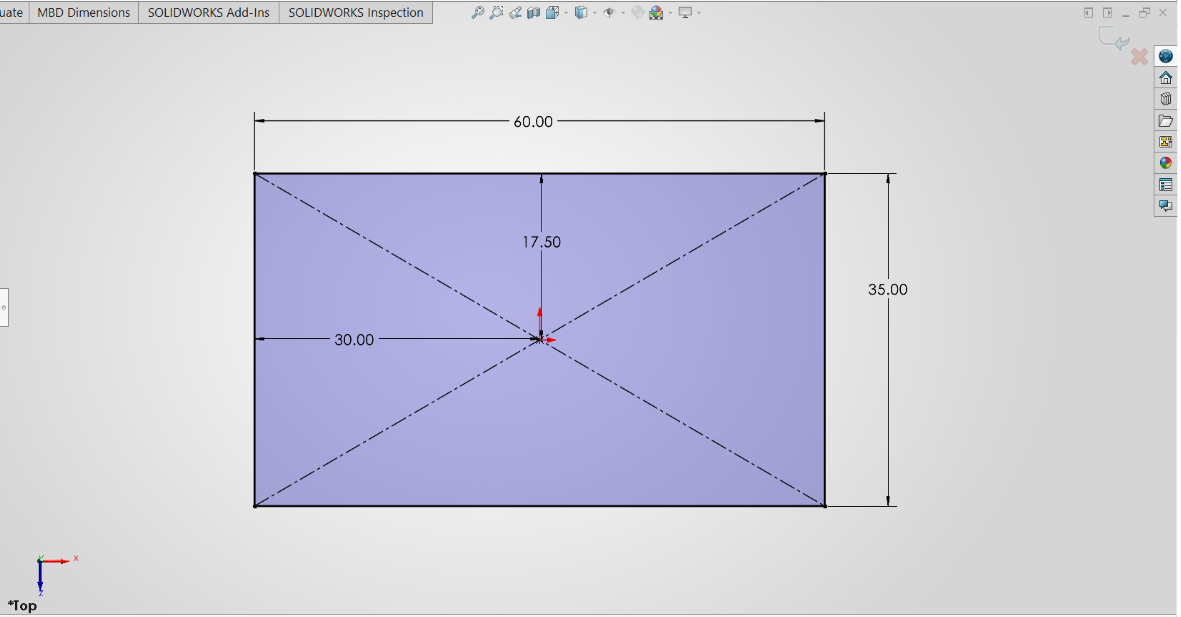
\includegraphics[width=\textwidth, keepaspectratio]{lab-01/assets/object-3/object-3-snap-1.png}
	\end{subfigure}
	\begin{subfigure}[b]{0.45\textwidth}
		\centering
		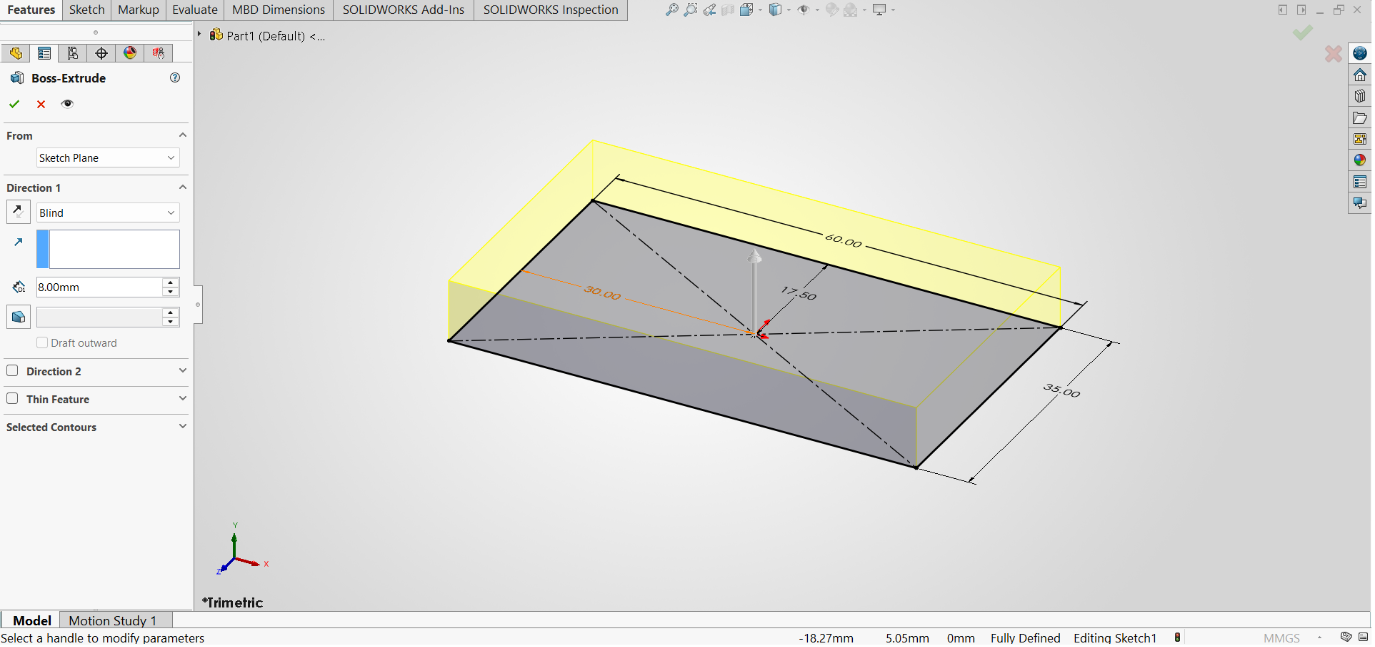
\includegraphics[width=\textwidth, keepaspectratio]{lab-01/assets/object-3/object-3-snap-2.png}
	\end{subfigure}
	\begin{subfigure}[b]{0.45\textwidth}
		\centering
		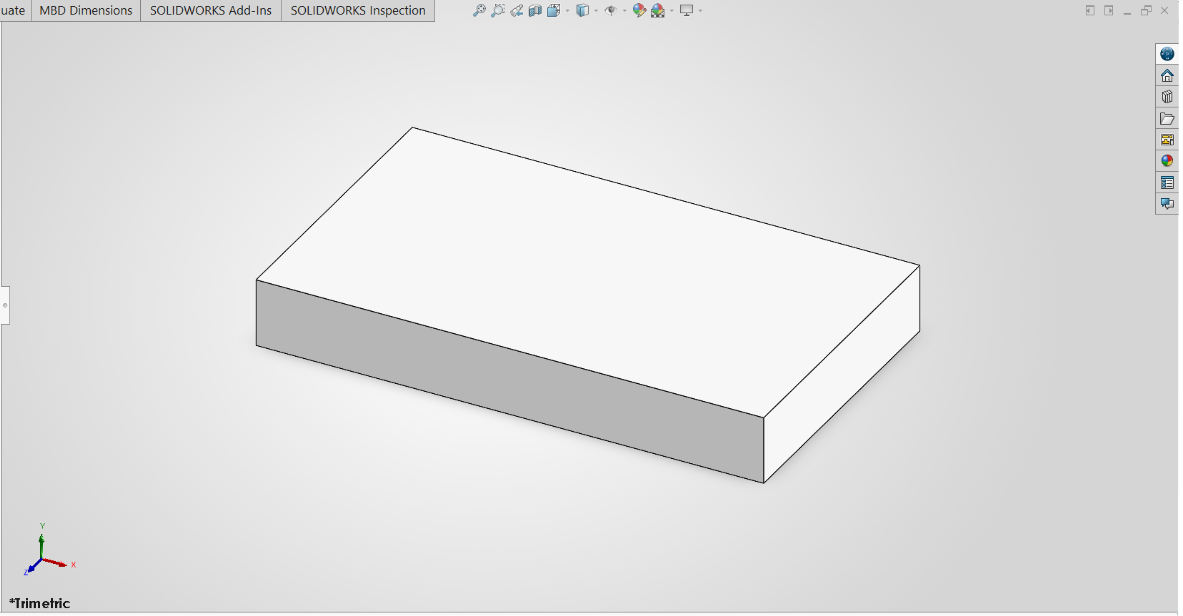
\includegraphics[width=\textwidth, keepaspectratio]{lab-01/assets/object-3/object-3-snap-3.png}
	\end{subfigure}
	\begin{subfigure}[b]{0.45\textwidth}
		\centering
		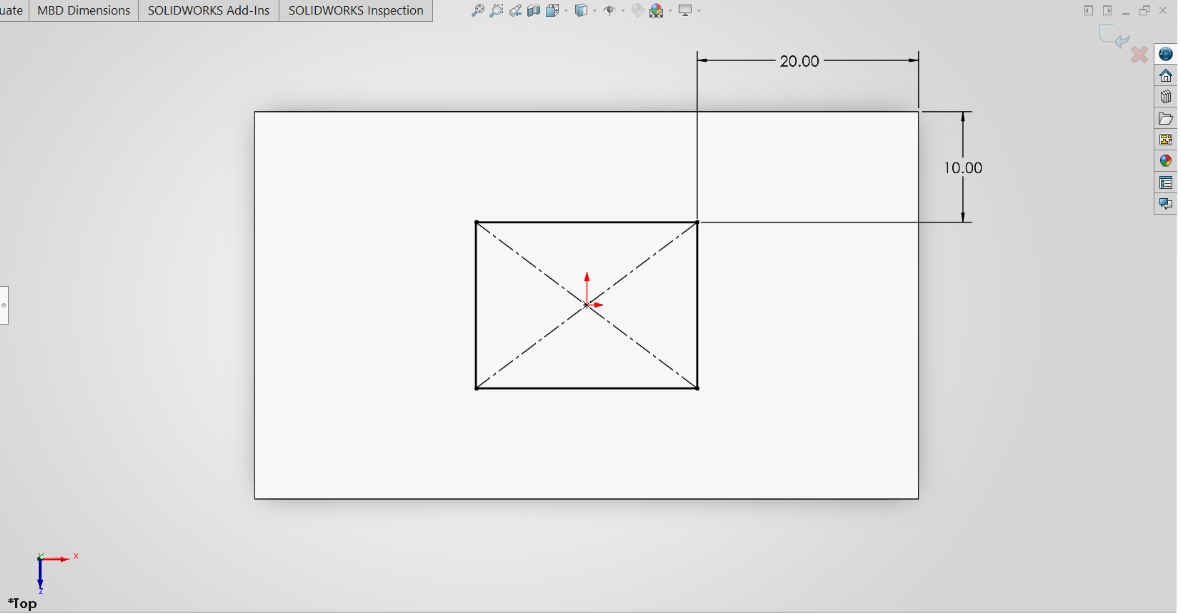
\includegraphics[width=\textwidth, keepaspectratio]{lab-01/assets/object-3/object-3-snap-4.png}
	\end{subfigure}
	\begin{subfigure}[b]{0.45\textwidth}
		\centering
		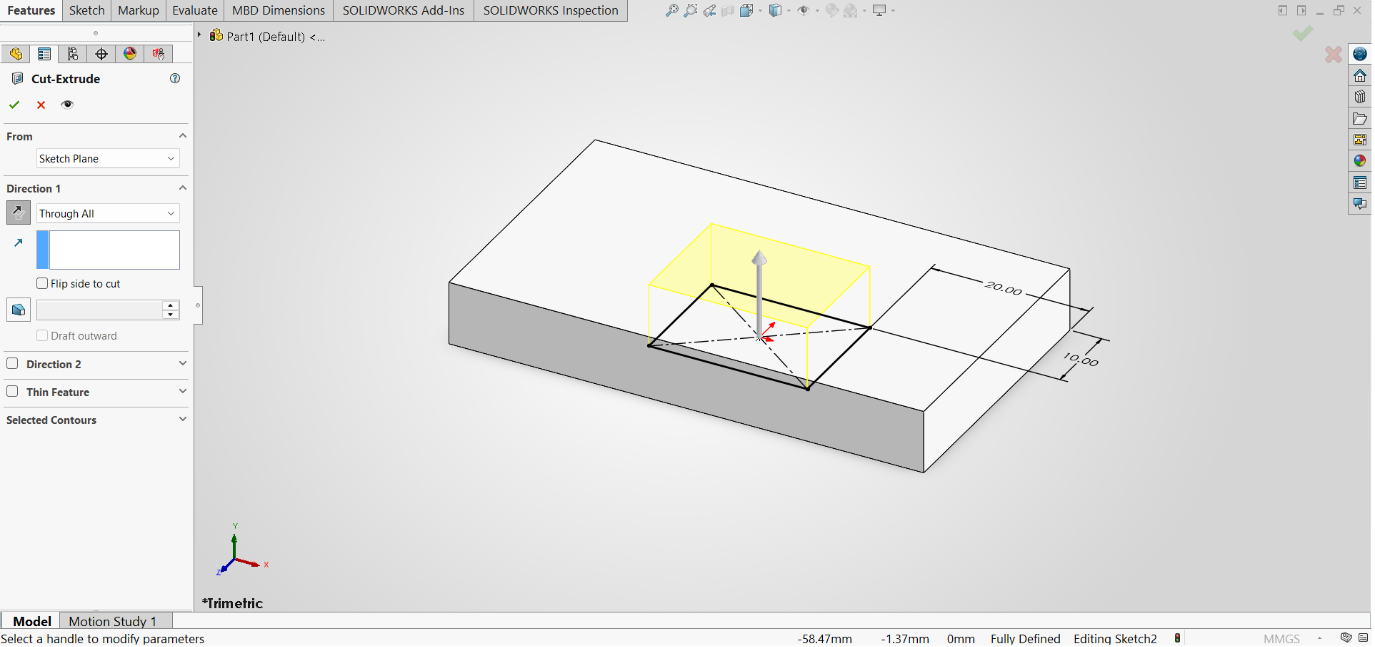
\includegraphics[width=\textwidth, keepaspectratio]{lab-01/assets/object-3/object-3-snap-5.png}
	\end{subfigure}
	\begin{subfigure}[b]{0.45\textwidth}
		\centering
		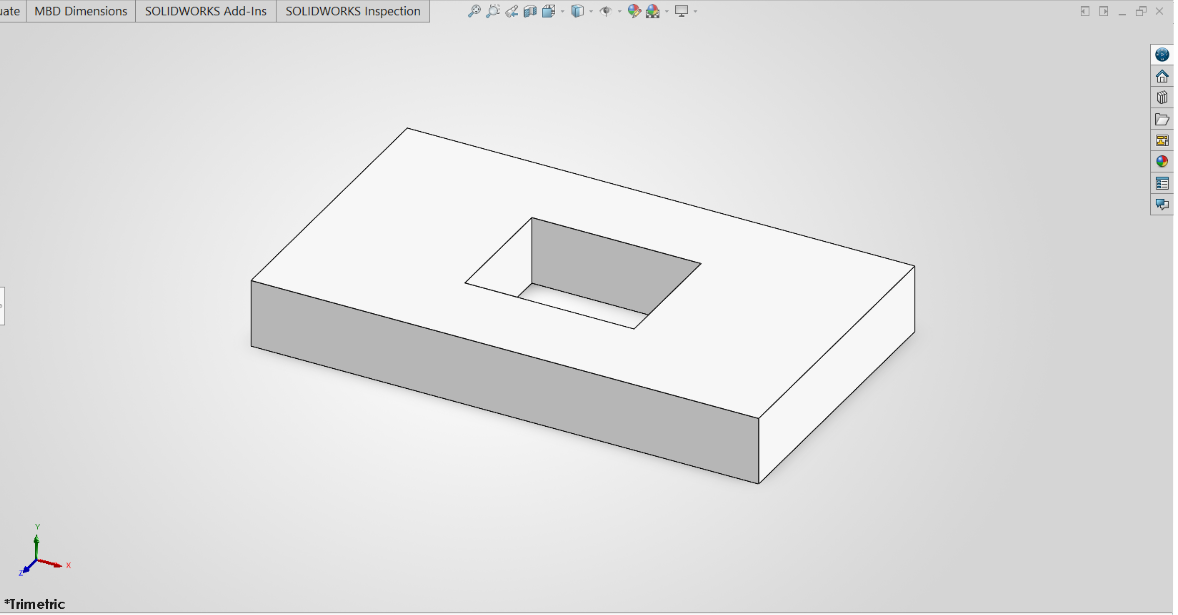
\includegraphics[width=\textwidth, keepaspectratio]{lab-01/assets/object-3/object-3-snap-6.png}
	\end{subfigure}
	\begin{subfigure}[b]{0.45\textwidth}
		\centering
		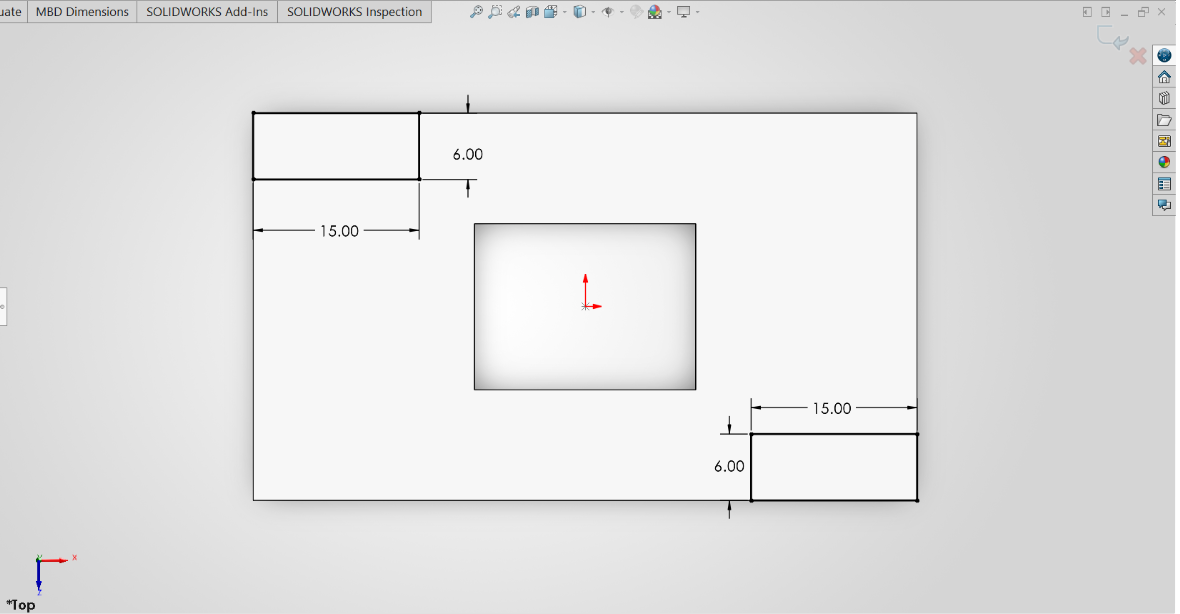
\includegraphics[width=\textwidth, keepaspectratio]{lab-01/assets/object-3/object-3-snap-7.png}
	\end{subfigure}
	\begin{subfigure}[b]{0.45\textwidth}
		\centering
		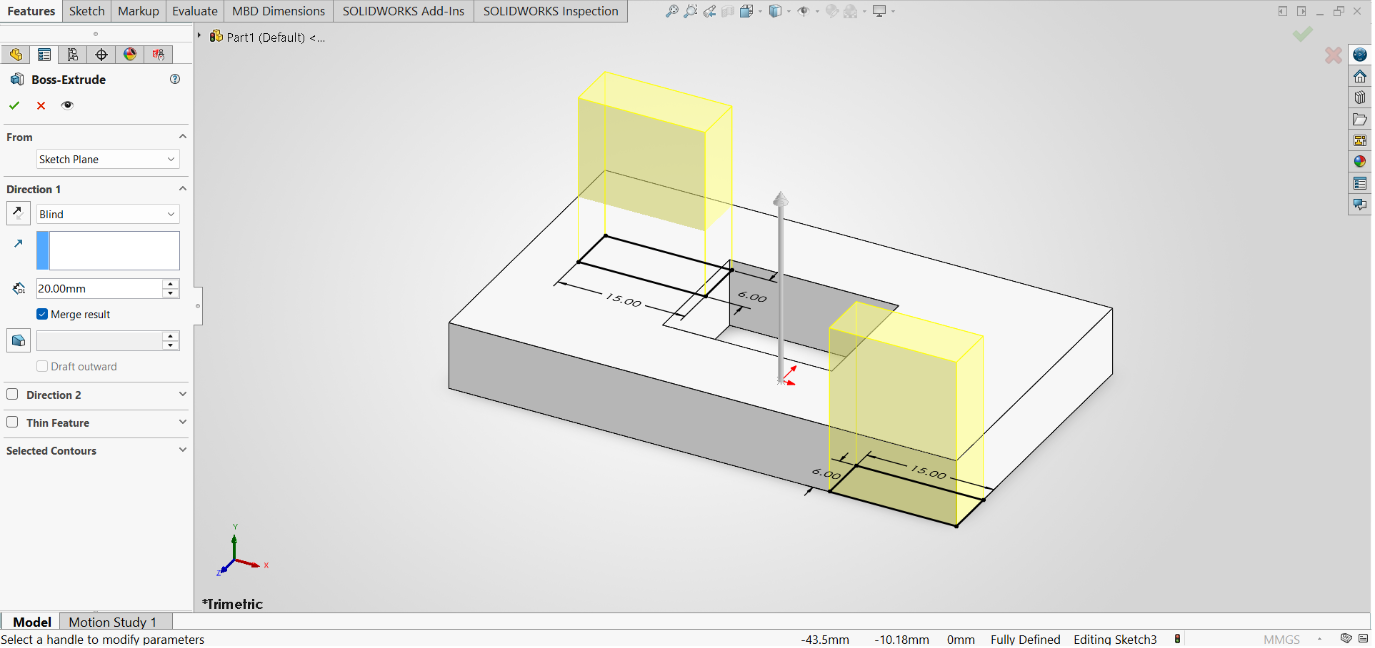
\includegraphics[width=\textwidth, keepaspectratio]{lab-01/assets/object-3/object-3-snap-8.png}
	\end{subfigure}
	\begin{subfigure}[b]{0.90\textwidth}
		\centering
		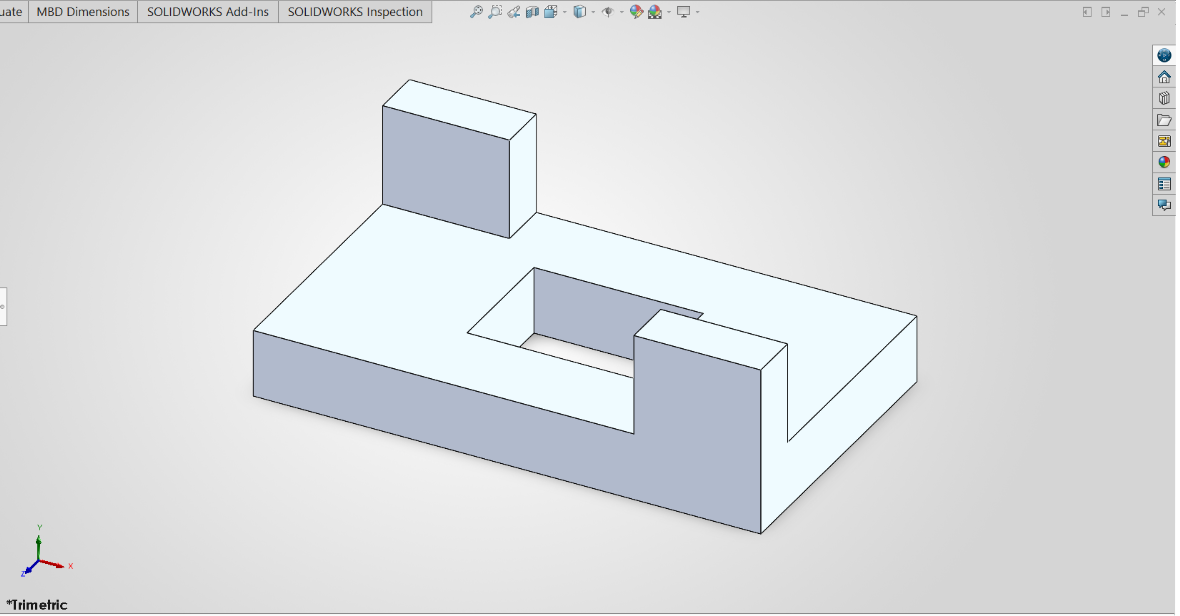
\includegraphics[width=\textwidth, keepaspectratio]{lab-01/assets/object-3/object-3-snap-9.png}
	\end{subfigure}

	\caption{Snapshots while Designing Object 3 in Solidworks}
	\label{lab01_object_3}
\end{figure}

